\documentclass{beamer}
\usepackage{polynom}
\usepackage{tikz}
\usepackage{soul}
\usepackage{xparse}
\usepackage{array}
\usepackage{longtable}

\title{HL Math Help}
\subtitle{Version 1}
\date{December 6 2020}
\institute[SST]{Student-to-Student Tutoring}

\usetheme{default}
\AtBeginSection{
    \begin{frame}
        \centering\Huge\Roman{section}.~\insertsectionhead
    \end{frame}
}
\AtBeginSubsection{
    \begin{frame}
        \centering\Large{\Roman{section}.\roman{subsection}.~\insertsubsectionhead}
    \end{frame}
}
% \setbeamertemplate{headline}{%
% \leavevmode%
%     \begin{beamercolorbox}[wd=\paperwidth,ht=0.5cm,sep=0.3cm]{palette quaternary}%
%        \large  \insertsectionhead \insertsubsectionhead
%     \end{beamercolorbox}%

    
% }
% \setbeamertemplate{navigation symbols}{}

\newcounter{step}

\renewcommand{\thestep}{\Roman{step}}
\NewDocumentCommand{\step}{o}{
    \par
    \stepcounter{step}
    \textbf{Step \thestep}
    \IfNoValueTF{#1}{ 
    }{
        \textbf{:~#1}
    }
    
}
% \newcommand{\step}[1][]{\stepcounter{step}\thestep :~#1}
\newcommand{\resetsteps}{\setcounter{step}{0}}

\begin{document}
    \begin{frame}
        \titlepage
    \end{frame}
    \foreach \x in {1,2,3,4,5,6,7} {%
        \begin{frame}
            \frametitle{Overview}
            \tableofcontents[sections=\x]
        \end{frame}
    }
    \section{Polynomial Theorems}
    \subsection{Factor Theorem}
    \begin{frame}
        If $c$ is a root of $p(x)$, $(x-c)$ is a factor of $p(x)$.
    \end{frame}
    \subsection{Remainder Theorem}
    \begin{frame}
        The remainder when $p(x)$ is divided by $c$ is $p(c)$.
    \end{frame}
    \subsection{Rational Root Theorem}
    \begin{frame}
        For the polynomial $p(x) = a_nx^2 + \cdots + a_0$, the rational roots are represented by $\frac{\text{factors}(a_0)}{\text{factors}(a_n)}$
        \begin{example}
            Given the polynomial $3x^3+4x^2+2x+7$, the possible rational roots can be expressed as:
            $$
                \text{p.r.z.} = \frac{\pm 1,~\pm 7}{\pm 1,~\pm 3}
            $$
            This should be represented as:
            $$
                \text{p.r.z.} = \left\{\pm 1,\pm\frac{1}{3},\pm 7,\pm\frac{7}{3}\right\}
            $$
        \end{example}
    \end{frame}
    \subsection{Complex Conjugate Root Theorem}
    \begin{frame}
        Complex roots always come in conjugate pairs.
        \begin{example}
            If $x-mi$ is a factor of $f(x)$, then $x+mi$ must also be a factor of $f(x)$.
        \end{example}
        \begin{alertblock}{N.B.}
            Always remember to state the theorem you are using!
        \end{alertblock}
    \end{frame}
    \subsection{Sum and Product of Roots}
    \begin{frame}
        Consider the following $n$th degree polynomial:
        $$
            p(x) = a_{n}x^n + a_{n-1}x^{n-1} + \cdots + a_{1}x^{1} + a_0
        $$
        The sum and product of roots can be found using the following formulae:
        \begin{columns}
            \begin{column}{.5\textwidth}
                \begin{eqnarray*}
                    \Sigma\text{Roots} & = & \frac{-a_{n-1}}{a_n}
                \end{eqnarray*}
            \end{column}
            \begin{column}{.5\textwidth}
                \begin{eqnarray*}
                    \Pi\text{Roots} & = & \frac{(-1)^{n}a_0}{a_n}
                \end{eqnarray*}
            \end{column}
        \end{columns}
    \end{frame}
    \section{Properties of Functions}
    \subsection{Even and Odd-Powered Polynomials}
    \begin{frame}
        \frametitle{Even-Powered Polynomials}
        Consider the Polynomial:
        $$
            p(x) = a_{n}x^n + \cdots + a_1x^1 + a_0
        $$
        If $n$ is an even number (i.e. if $2 \vert n$), are two scenarios to consider: 
        \begin{enumerate}
            \item Even-powered polynomials when $a_n < 0$ go from the bottom left, do something wonky, and come down on the bottom right.
            \item Even-powered polynomials when $a_n > 0$ go from the top left, do something wonky, and come down on the top right.
        \end{enumerate}
    \end{frame}
    \begin{frame}
        \begin{example}
            \begin{figure}
                \caption{$x^2$ when $a_n < 0$} 
                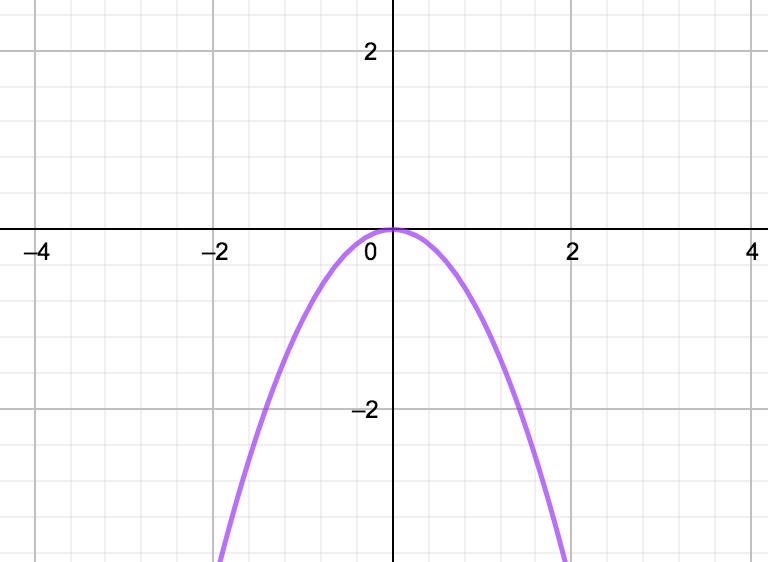
\includegraphics[scale=0.3]{images/x2-ls-0.png}
            \end{figure}
        \end{example}
    \end{frame}
    \begin{frame}
        \begin{example}
            \begin{figure}
                \caption{$x^2$ when $a_n > 0$} 
                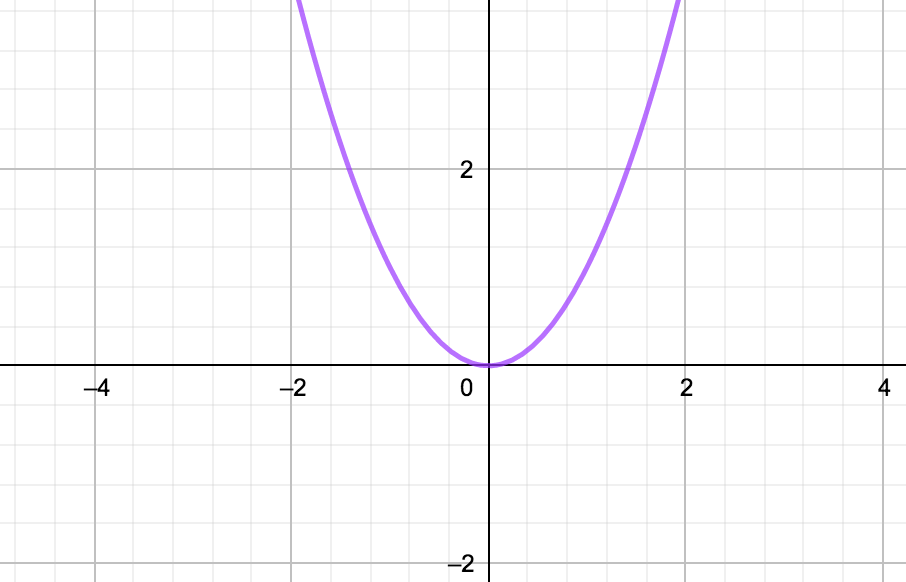
\includegraphics[scale=0.3]{images/x2-gtd-0.png}
            \end{figure}
        \end{example}
    \end{frame}
    \begin{frame}
        \frametitle{Odd-Powered Functions}
        Consider the same polynomial:
        $$
            p(x) = a_{n}x^n + \cdots + a_1x^1 + a_0
        $$
        If $n$ is an odd number, there are also two scenarios to consider: 
        \begin{enumerate}
            \item Odd-powered polynomials when $a_n > 0$ go from the bottom left, do something wonky, and come up on the top right.
            \item Odd-powered polynomials when $a_n < 0$ go from the top left, do something wonky, and come down on the bottom right.
        \end{enumerate}
    \end{frame}
    \begin{frame}
        \begin{example}
            \begin{figure}
                \caption{$x$ when $a_0 < 0$}
                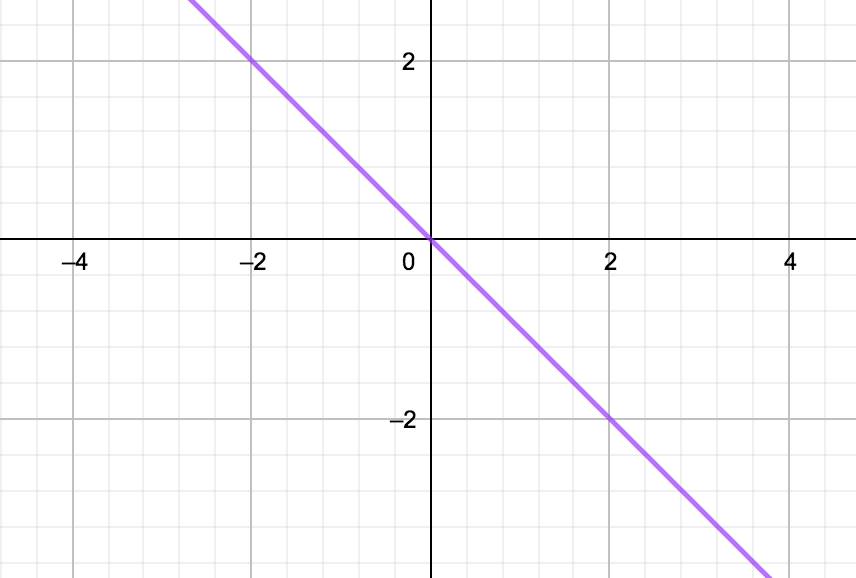
\includegraphics[scale=0.3]{images/x-nega.png}
            \end{figure}
        \end{example}
    \end{frame}
    \begin{frame}
        \begin{example}
            \begin{figure}
                \caption{$x$ when $a_0 > 0$}
                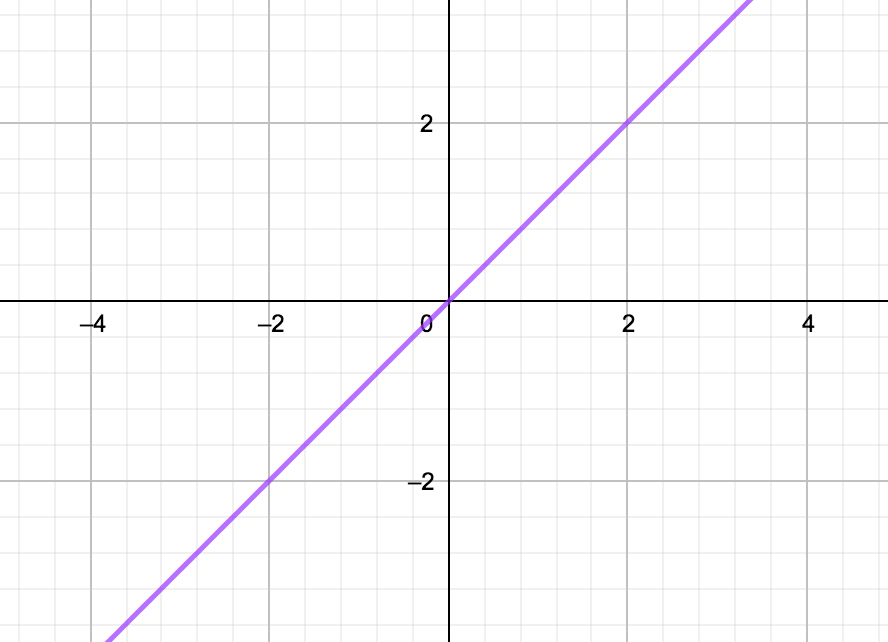
\includegraphics[scale=0.3]{images/x-posi.png}
            \end{figure}
        \end{example}
    \end{frame}
    \subsection{Even and Odd Functions}
    \begin{frame}
        \frametitle{The Odd Function}
        An odd function is a function with the following property:
        $$f(x)=-f(-x)$$
        This essentially means it is symmetrical over the $y=x$ line.
        \begin{alertblock}{N.B.}
            An \emph{odd function} is not the same as an \emph{odd-powered polynomial}!
        \end{alertblock}
    \end{frame}
    \begin{frame}
        \begin{example}
            The $\sin$ function is an example, as it is symmetrical over the $y=x$ line, as shown in the figure below:
            \begin{figure}
                \caption{The $sin$ function is symmetrical over the $y=x$ line}
                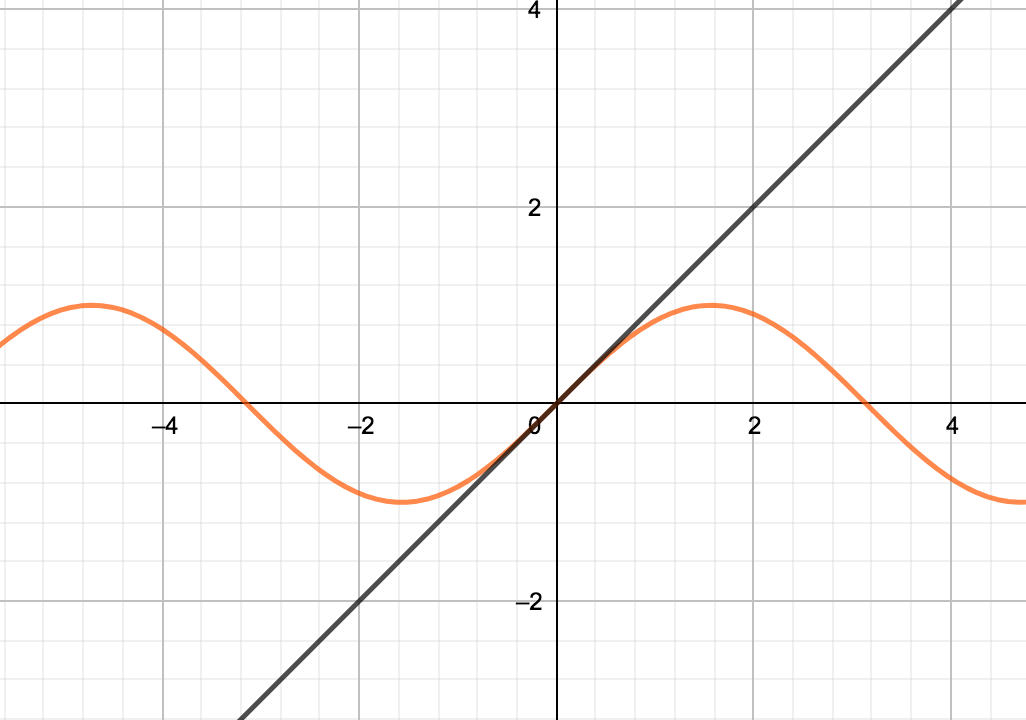
\includegraphics[scale=0.2]{images/sin.png}
            \end{figure}
        \end{example}
    \end{frame}
    \begin{frame}
        \frametitle{The Even Function}
        An even function is a function with the following property:
        $$f(x)=f(-x)$$
        This essentially means it is symmetrical over the $y$ axis.
    \end{frame}
    \begin{frame}
        \begin{example}
            \begin{figure}
                \caption{The $\cos$ function}
                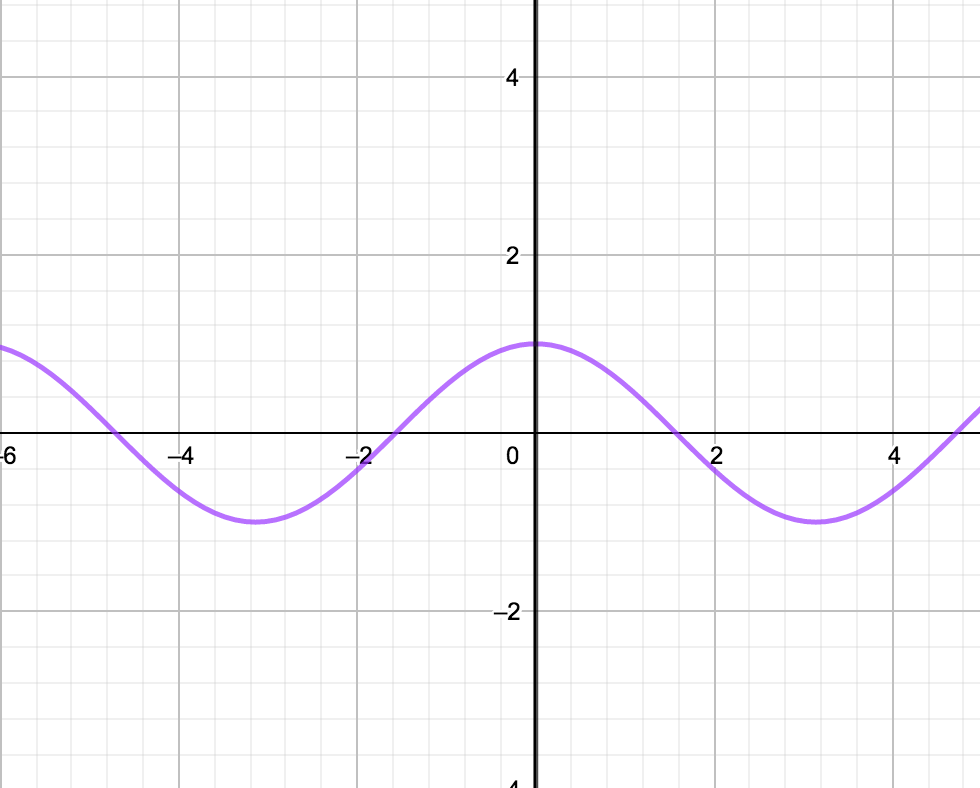
\includegraphics[scale=0.3]{images/cos.png}
            \end{figure}
        \end{example}
    \end{frame}
    \begin{frame}
        \begin{example}
            \begin{figure}
                \caption{The $x^2$ function}
                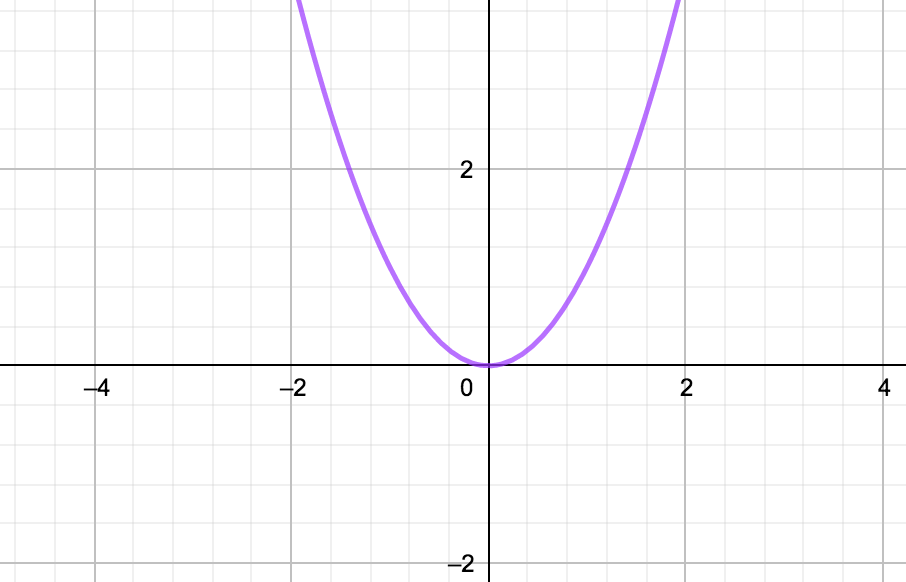
\includegraphics[scale=0.3]{images/x2-gtd-0.png}
            \end{figure}
        \end{example}
    \end{frame}
    \begin{frame}
        \begin{example}
            \begin{figure}
                \caption{The $\left\lvert x \right\rvert$ function}
                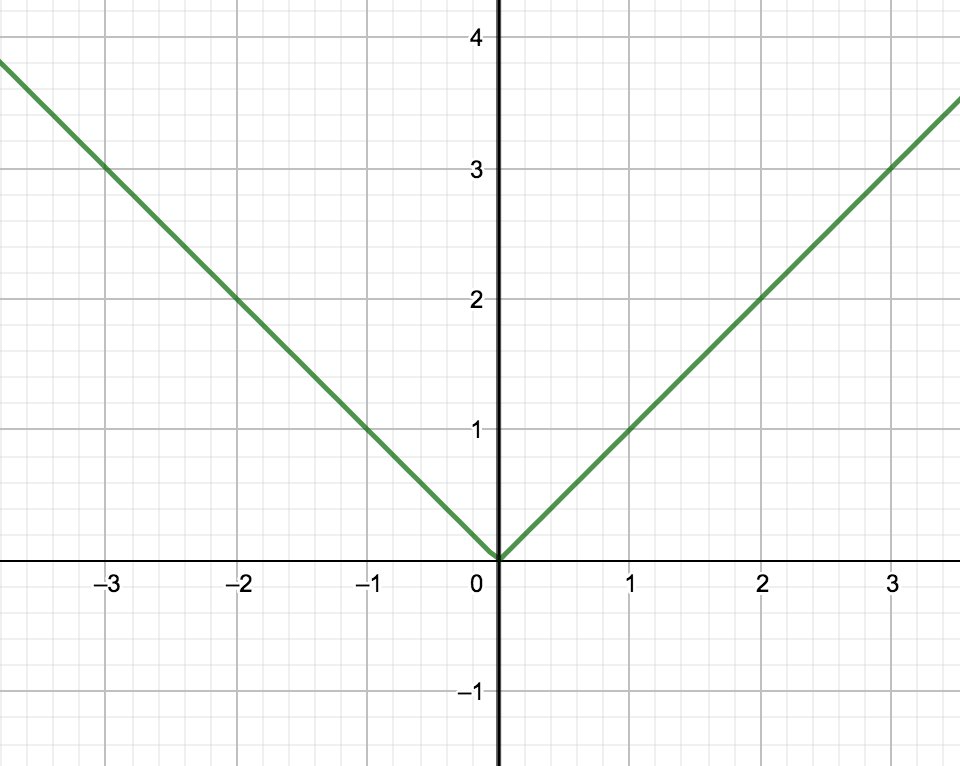
\includegraphics[scale=0.3]{images/absx.png}
            \end{figure}
        \end{example}
    \end{frame}
    \begin{frame}
        \begin{alertblock}{N.B.}
            Because an even function is symmetrical over the $y$ axis, a vertical translation keeps it an even function. That said, a horizontal translation makes it no longer an even function. This means that $x^2$ and $x^2+1$ are both even functions, though $(x+1)^2$ is not.
        \end{alertblock}
    \end{frame}
    \subsection{Function Transformations}
    \begin{frame}
        \frametitle{Formulae}
        Given a function of the form:
        $$
            g(x) = af(bx-h) + k
        $$
        Any of its transformed coordinates can be determined by the following formula:
        $$
        (x,y) \mapsto \left(\frac{x}{b} + h , ay + k\right)
        $$
        Of course, an alternate method is to use logic.
    \end{frame}
    \begin{frame}
        \frametitle{Example Question}
        Given the graph of the function $f(x)$ below, determine the coordinates of the local extrema in the transformed function $g(x)=2f(x-3)+1$.
        \begin{figure}
            \caption{Mystery Function $f(x)$}
            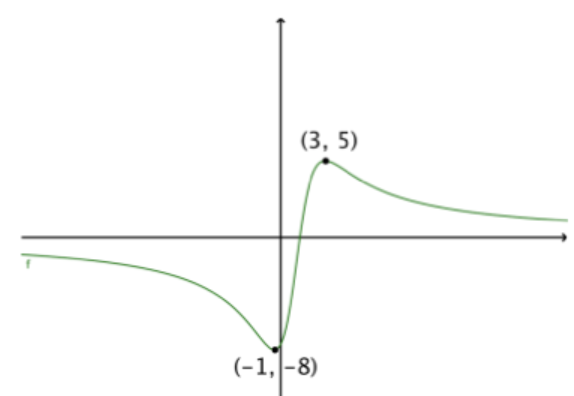
\includegraphics[scale=0.3]{images/mystery-f(x).png}
        \end{figure}
    \end{frame}
    \begin{frame}[allowframebreaks]
        We start by noting down all relevant information about the function:
        \begin{table}
            \begin{tabular}{c|c}
                $a$ & 2 \\
                $b$ & 1 \\
                $h$ & 3 \\
                $k$ & 1 \\
            \end{tabular} 
        \end{table}
        Then we apply the formula for point $(3,5)$:
        \begin{eqnarray*}
            (x, y) & \mapsto & \left(\frac{x}{b} + h, ay + k \right) \\
            (3, 5) & \mapsto & \left(3 + 3, 10 + 1\right) \\
            & \mapsto & \left(6, 11\right) \\
        \end{eqnarray*}
        And for point $(-1,-8)$:
        \begin{eqnarray*}
            (x, y) & \mapsto & \left(\frac{x}{b} + h, ay + k \right) \\
            (-1, -8) & \mapsto & \left(2, -15\right) \\
        \end{eqnarray*}
    \end{frame}
    \section{Derivatives}
    \subsection{Power Rule}
    \begin{frame}
        To find the derivative of $f(x)$, for each term, you multiply the coefficient by the power, make that the new coefficient, subtract one from the exponent, and make that the new exponent. \alert{As a result, constant terms are ignored, but negative exponents are not!}
        \begin{example}
            Given $f(x)=5x^3+3x^2+2x+1$, the derivative is $f'(x)=15x^2 + 6x + 2$.
        \end{example}
        \begin{definition}
            The derivative of $f(x)$ is often written as $f'(x)$.
        \end{definition}
    \end{frame}
    \section{Chaos Theory}
    \subsection{Fixed Points}
    \begin{frame}
        A fixed point is when the function is equal to itself (i.e. the point is "trapped"). Fixed points are found by solving for $f(x)=x$ (i.e. the intersection between the function and the $y=x$ line).
    \end{frame}
    \begin{frame} 
        \begin{example}
            The fixed points of $x^2-2$ would be:
            \begin{eqnarray*}
                x^2 - 2 - x & = & 0 \\
                (x-2)(x+1) & = & \\
                x & \in & \left\{-1,2\right\}
            \end{eqnarray*}
            So the fixed points are -1 and 2. 
            This is also shown by the graph:
            \begin{figure}
                \centering
                \caption{Fixed points of $x^2-2$}
                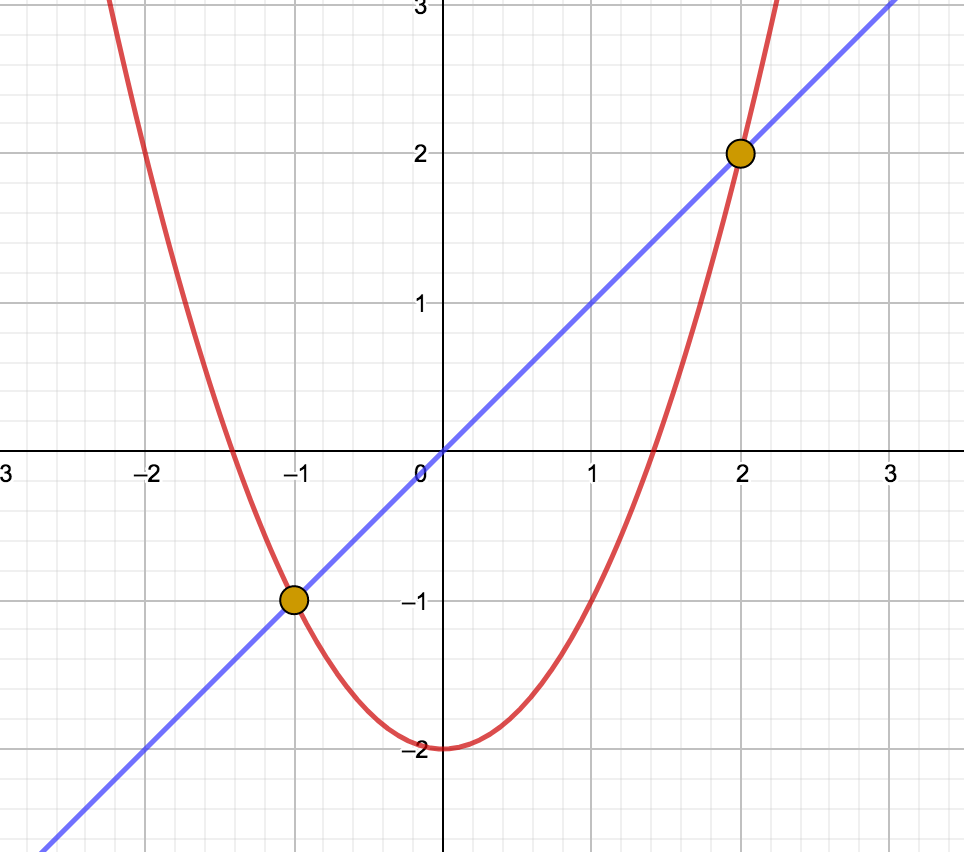
\includegraphics[scale=.2]{images/fixed-points-1.png}
            \end{figure}
        \end{example} 
    \end{frame}
    \subsection{Stability}
    \begin{frame}
        The stability of a fixed point can be determined using the derivative of the original function. Let $x_{\star}$ be a fixed point of $f(x)$. Let $g=|f'(x_\star)|$. If $g>1$, it is unstable and repelling. If $g=1$, it is neutral. If $g<1$, it is stable and attracting.
        \begin{example}
            The fixed points of $f(x)=x^2-2$ are $x_\star \in \left\{-1,2\right\}$. $f'(x)=2x$, and let $g(x)=|f'(x)|$. For -1, $g(-1)=2$, which is greater than 1. $g(2)=4$, which is greater than 1. Both fixed points are unstable and repelling.
        \end{example}
    \end{frame}
    \subsection{Cobweb Method}
    \begin{frame}[shrink]
        The cobweb method is a technique to find the fixed points of any given function. Essentially, you follow this procedure:
        \setbeamercovered{transparent}
        \begin{columns}
            \begin{column}{.5\textwidth}
                \begin{enumerate}[I]
                    \only<1-3>{
                        \item<1-> Draw the the $y=x$ line on a cartesian plane. 
                        \item<2-> Draw the function (we will use the example from earlier, $f(x)=x^2-2$)
                        \item<3-> Choose a point on the $x$-axis near the fixed point you are testing (we are testing fixed point $x_\star=2$).
                    }
                    \only<4-6>{
                        \setcounter{enumi}{3}
                        \item<4-> Draw a line from that point to the function.
                        \item<5-> Draw a line from the function to the $y=x$ line.
                        \item<6-> Draw a line from the $y=x$ line to the function (in this case it converges already).
                    }
                \end{enumerate}
            \end{column}
            \begin{column}{.5\textwidth}
                \begin{figure}
                    \only<1>{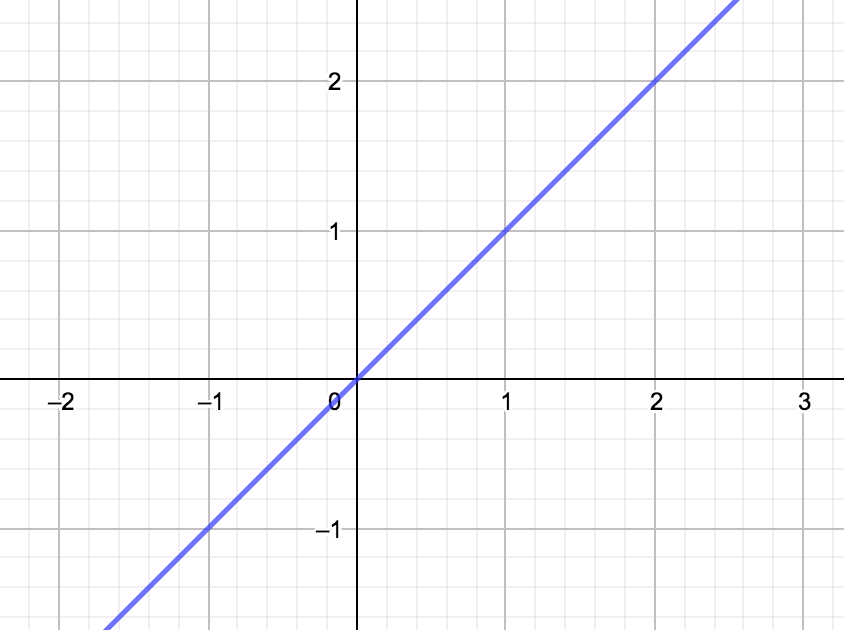
\includegraphics[scale=0.3]{images/y=x.png}}
                    \only<2>{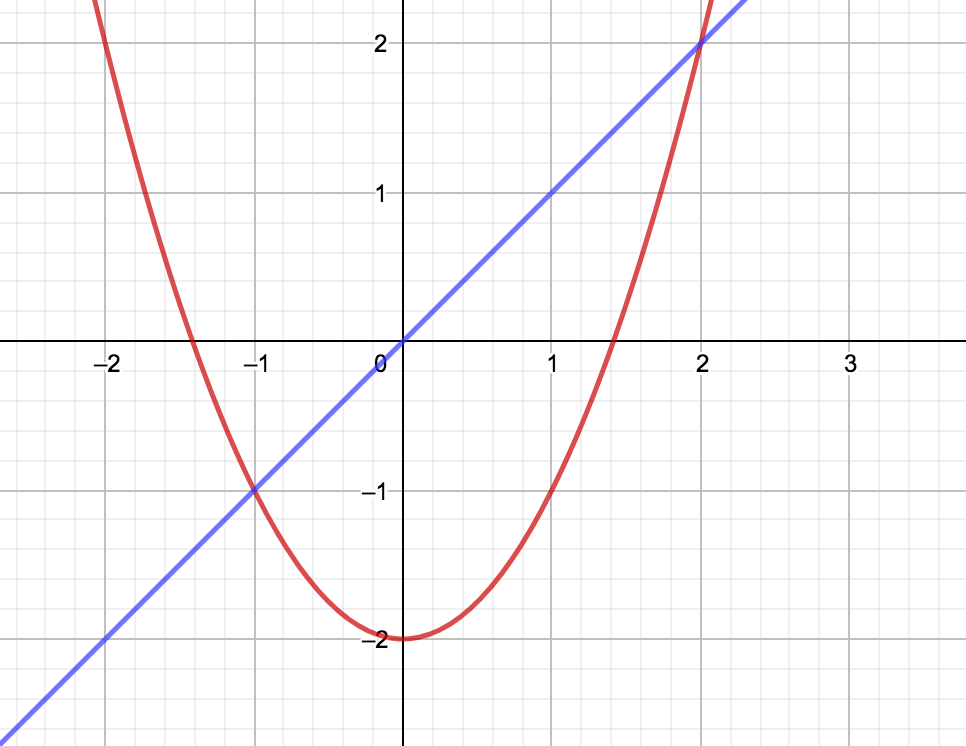
\includegraphics[scale=0.3]{images/func-1.png}}
                    \only<3>{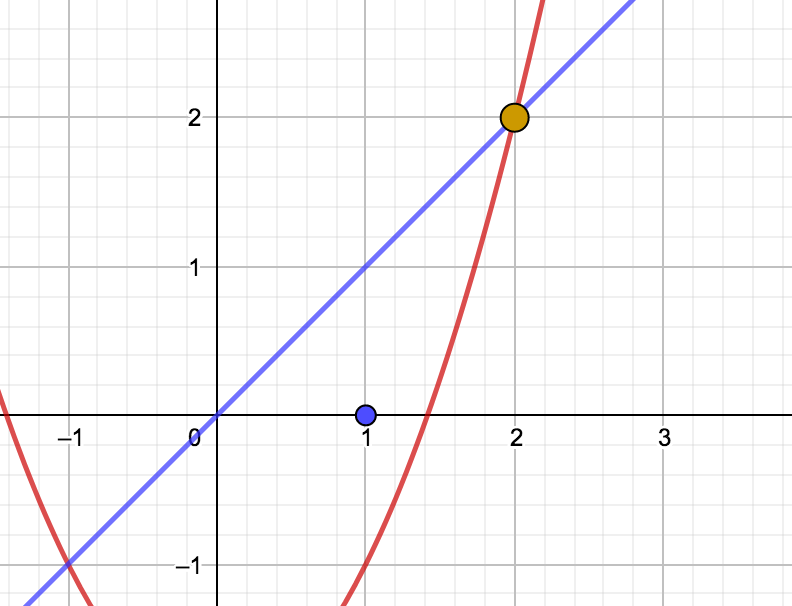
\includegraphics[scale=0.3]{images/chose-pnt-1.png}}
                    \only<4>{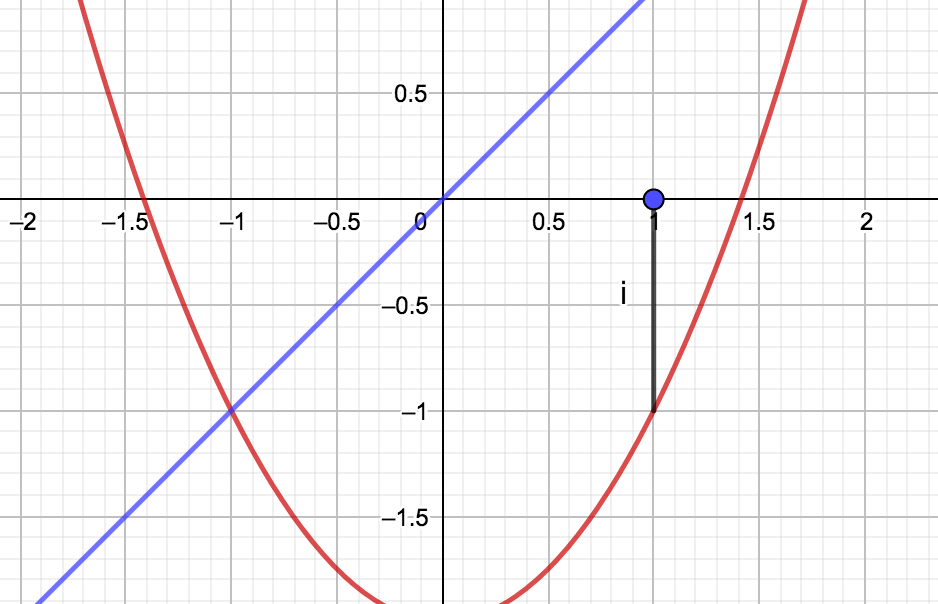
\includegraphics[scale=0.3]{images/follow-pnt-1.png}}
                    \only<5-6>{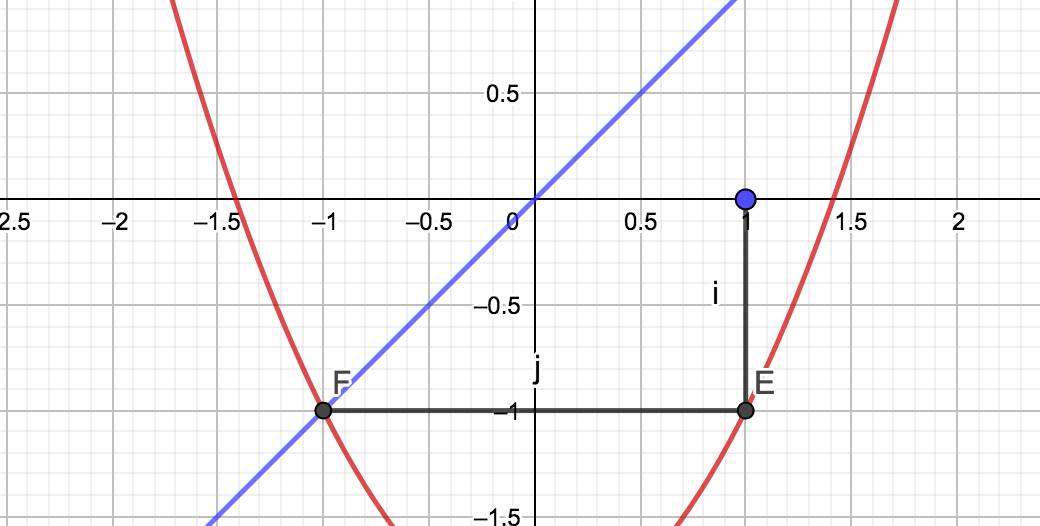
\includegraphics[scale=0.3]{images/follow-pnt-2.png}}
                \end{figure}
            \end{column}
        \end{columns}
    \end{frame}
    \begin{frame}
        Repeat this process until you can see whether
        \begin{enumerate}
            \item It diverges (unstable and repelling)
            \item It converges to the point (stable and attracting)
            \item It behaves in a chaotic way (neutral)
        \end{enumerate}
    \end{frame}
    \subsection{n-cycles}
    \begin{frame}
        \only<1>{
            To find an $n$-cycle, all one must do is plug the function into itself $n$ times. An $n^{\text{th}}$ cycle is often written as $^nf(x)$, for a given function $f(x)$. \par
            It is important to note that all one-cycles are \textbf{trivial} $n$-cycles. This means that they will appear as $n$-cycles, even if really, they are one-cycles. \par
            Also note that an $n$-cycle means that it gets stuck into a loop of sorts, where the function alternates between the values in the cycle.
        }
        \only<2->{
            \begin{example}
                \only<2>{
                    Find all 2-cycles of $f(x)=x^2-2$. To to so, we must compute $f(f(x))-x=0$.
                    \begin{eqnarray*}
                        ^2f(x)-x&=&0 \\
                        f(f(x))-x&=&0 \\
                        (x^2-2)^2-2-x&=&0 \\
                        x^4-4x^2-x+2 & = & 0 \\
                    \end{eqnarray*}
                }
                \only<3>{
                    Fortunately, we know that all one-cycles are trivial $n$-cycles, so $x^2-x-2$ is a root of $x^4-4x^2-x+2$. To find the other roots, we simply divide the two and factor the resulting quadratic:
                    \polylongdiv{x^4-4x^2-x+2}{x^2-x-2}
                }
                \only<4>{
                    Now, we apply the quadratic formula:
                    \begin{eqnarray*}
                        x^2-x-1 & = & 0 \\
                        x & = & \frac{-1\pm\sqrt{1-4(1)(-1)}}{2} \\
                        x & = & \frac{-1 \pm\sqrt{5}}{2}
                    \end{eqnarray*}
                    Therefore, the \textbf{trivial} 2-cycles are -1 and 2, and the \textbf{nontrivial} 2-cycles are $\frac{-1 + \sqrt{5}}{2}$ and $\frac{-1 - \sqrt{5}}{2}$
                }
            \end{example}
        }
    \end{frame}
    \section{Advanced Rational Functions}
    \subsection{Inequalities}
    \begin{frame}
        What is the solution to the following?
        $$
            \frac{x^2 + 5x}{x^2 - 4} > 0
        $$
    \end{frame}
    \begin{frame}
        Start by factoring to get:
        $$
            \frac{x(x+5)}{(x-2)(x+2)} > 0
        $$
        Note down some of the properties
        \begin{table}
            \centering
            \begin{tabular}{ll}
                Zeroes: & $x=0$ \\
                & $x=-5$ \\
                Restrictions: & $x\neq-2$ \\
                & $x\neq 2$
            \end{tabular}
        \end{table}
    \end{frame}
    \begin{frame}
        Now, note down these values on a number line, and identify the sections that must be tested: 
        \begin{table}
            \begin{tabular}{ccccccccc}
                \textcolor{red}{\textbf<2>{A}} & -5 & \textcolor{red}{\textbf<3>{B}} & -2 & \textcolor{red}{\textbf<4>{C}} & 0 & \textcolor{red}{\textbf<5>{D}} & 2 & \textcolor{red}{\textbf<6>{E}} \\
                \hline
            \end{tabular}
        \end{table}
        \begin{columns}
            \only<2>{
                \begin{column}{.5\textwidth}
                    Testing for \textcolor{red}{\textbf{A}} \\
                    \begin{eqnarray*}
                        x & = & -6 \\
                        & = & \frac{-6(-6+5)}{(-6-2)(-6+2)} \\
                        & = & \frac{-\cdot -}{- \cdot -} \\
                        & = & + \\
                        + & > & 0 \\
                    \end{eqnarray*}
                \end{column}
                \begin{column}{.5\textwidth}
                    This section does not work.
                \end{column}
            }
            \only<3>{
                \begin{column}{.5\textwidth}
                    Testing for \textcolor{red}{\textbf{B}} \\
                    \begin{eqnarray*}
                        x & = & -3 \\
                        & = & \frac{-3(-3+5)}{(-3-2)(-3+2)} \\
                        & = & \frac{- \cdot +}{- \cdot -} \\
                        & = & -\\
                        - & < & 0\\
                    \end{eqnarray*}
                \end{column}
                \begin{column}{.5\textwidth}
                    This section works.
                \end{column}
            }
            \only<4>{
                \begin{column}{.5\textwidth}
                    Testing for \textcolor{red}{\textbf{C}} \\
                    \begin{eqnarray*}
                        x & = & -1 \\
                        & = & \frac{-1(-1+5)}{(-1-2)(-1+2)} \\
                        & = & \frac{- \cdot +}{- \cdot +} \\
                        & = & + \\
                        + & > & 0\\
                    \end{eqnarray*}
                \end{column}
                \begin{column}{.5\textwidth}
                    This section does not work.
                \end{column}
            }
            \only<5>{
                \begin{column}{.5\textwidth}
                    Testing for \textcolor{red}{\textbf{D}} \\
                    \begin{eqnarray*}
                        x & = & 1 \\
                        & = & \frac{1(1+5)}{(1-2)(1+2)} \\
                        & = & \frac{+ \cdot +}{- \cdot +} \\
                        & = & - \\
                        - & < & 0\\
                    \end{eqnarray*}
                \end{column}
                \begin{column}{.5\textwidth}
                    This section works.
                \end{column}
            }
            \only<6>{
                \begin{column}{.5\textwidth}
                    Testing for \textcolor{red}{\textbf{E}} \\
                    \begin{eqnarray*}
                        x & = & 3 \\
                        & = & \frac{3(3+5)}{(3-2)(3+2)} \\
                        & = & \frac{+ \cdot +}{+ \cdot +} \\
                        & = & + \\
                        + & > & 0\\
                    \end{eqnarray*}
                \end{column}
                \begin{column}{.5\textwidth}
                    This section does not work.
                \end{column}
            }
        \end{columns}
        \only<7>{
            \centering
            In conclusion, $x < 0$ so long as $x \in~]-5,-2[~\cup~]0,2[$
        }
    \end{frame}
    \section{Sequences and Series}
    \subsection{basic Formulae}
    \begin{frame}
        \frametitle<1>{Geometric Sequence}
        Let $a = {a_1, a_2, a_3, a_4, \cdots, a_n}$ where there are $n$ terms. 
        \only<1>{
            If each element is $r$ times the previous, the \textbf{sum} is:
            $$
                S_n = a_1\frac{1-r^n}{1-r}
            $$
            The \textbf{recursive formula} is:
            $$
                a_n = a_{n-1} \cdot r
            $$
            The \textbf{closed formula} is:
            $$
                a_n = a_{1} \cdot r^{n-1}
            $$
        } 
        \frametitle<2>{Algebraic Sequence}
        \only<2>{
            If each element is $d$ more than the previous, the \textbf{sum} is:
            $$
                S_n = n \left(\frac{a_1 + a_n}{2}\right)
            $$
            The \textbf{recursive formula} is:
            $$
                a_n = a_{n-1} + d
            $$
            The \textbf{closed formula} is:
            $$
                a_n = a_1 + d(n-1)
            $$
        }
    \end{frame}
    \section{Mathematical Induction}
    \begin{frame}
        \frametitle{Example Question}
        Use mathematical induction to prove that $5^n + 3^n \geq 2^{2n+1};~\forall n \in \mathbb{Z}^\star$ 
    \end{frame}
    \begin{frame}[allowframebreaks]
        \step
        $$
            \text{let}~p(n):~5^n+3^n \geq 2^{2n+1};~\forall n \in \mathbb{Z}^\star
        $$
        \step
        \begin{eqnarray*}
            p(1):~5 + 3& \geq &2^3 \\
            8 & \geq & 8
        \end{eqnarray*}
        $p(1)$ is true
        \step
        $$
            p(k):~5^k + 3^k \geq 2^{2k+1}
        $$
        \step
        $$
            p(k+1):~5^{k+1} + 3^{K+1} \stackrel{?}{\geq} 2^{2k+3};~\forall k \in \mathbb{Z}^\star 
        $$
        \begin{table}
            \renewcommand{\arraystretch}{1.5}
            \begin{longtable}{lm{4cm}}
                $LS = 5^{k+1} + 3^{k+1} $ & Start on the left side \\
                $5^k\cdot 5 + 3^k \cdot$ & Expand. \\
                $\geq (2^{2k+1} - 3^k)\cdot 5 + 3^k \cdot 3$ & By the Inductive hypothesis, we have that if $5^k + 3^k \geq 2^{2k+1}$, $5^k \geq 2^{2k+1} - 3^k$ \\
                $=5\cdot 2^{2k+1} - 5 \cdot 3^k + 3 \cdot 3^k$ & Simplify. \\
                $= 5 \cdot 2^{2k+1} - 2\cdot3^k $ & \\
                $\geq 5\cdot 2^{2k+1} - 2 \cdot 4^k$ & Because $-3^k \geq -4^k$ (notice the brackets and watch out for negative signs). \\
                $=5\cdot 2^{2k+1} -2 \cdot 2^2k$ & \\
                $=5\cdot 2^{2k+1} - \cdot 2^{2k + 1}$ & Because $4 = 2^2$ \\
                $= 4\cdot 2^{2k+1}$ & Simplify \\
                $= 2^{2k+3}$ & Because $4 = 2^2$ \\
                $= RS$ & This is equal to the right side \\
            \end{longtable}
        \end{table}
        \step
        By the principle of mathematical induction, $p(x)$ is true.
        $$\qed$$
    \end{frame}
\end{document}